%%
%% This is file `sample-sigconf.tex',
%% generated with the docstrip utility.
%%
%% The original source files were:
%%
%% samples.dtx  (with options: `sigconf')
%% 
%% IMPORTANT NOTICE:
%% 
%% For the copyright see the source file.
%% 
%% Any modified versions of this file must be renamed
%% with new filenames distinct from sample-sigconf.tex.
%% 
%% For distribution of the original source see the terms
%% for copying and modification in the file samples.dtx.
%% 
%% This generated file may be distributed as long as the
%% original source files, as listed above, are part of the
%% same distribution. (The sources need not necessarily be
%% in the same archive or directory.)
%%
%% The first command in your LaTeX source must be the \documentclass command.
\documentclass[sigconf]{acmart}

%=================================================================
%====ADDITIONAL PACKAGES & SETTINGS FROM THE ORIGINAL TEMPALTE====
\usepackage{import} % to use \import{../../../content-tex/}{abstract}
\usepackage{todonotes} % USAGE: \todo[inline]{is there a better example from X topic?}
\usepackage{lipsum}  % USAGE \lipsum[2-4]

%%
%% \BibTeX command to typeset BibTeX logo in the docs
\AtBeginDocument{%
  \providecommand\BibTeX{{%
    \normalfont B\kern-0.5em{\scshape i\kern-0.25em b}\kern-0.8em\TeX}}}

%% Rights management information.  This information is sent to you
%% when you complete the rights form.  These commands have SAMPLE
%% values in them; it is your responsibility as an author to replace
%% the commands and values with those provided to you when you
%% complete the rights form.
\setcopyright{acmcopyright}
\copyrightyear{2018}
\acmYear{2018}
\acmDOI{10.1145/1122445.1122456}

%% These commands are for a PROCEEDINGS abstract or paper.
\acmConference[Woodstock '18]{Woodstock '18: ACM International Conference of Human-Robot Interaction}{8 March 2021}{Online}
\acmBooktitle{Woodstock '18: ACM International Conference of Human-Robot Interaction,
8 March 2021, Online}
\acmPrice{15.00}
\acmISBN{978-1-4503-XXXX-X/18/06}

\graphicspath{{../figures}} %goes to path: figures/

%%
%% Submission ID.
%% Use this when submitting an article to a sponsored event. You'll
%% receive a unique submission ID from the organizers
%% of the event, and this ID should be used as the parameter to this command.
%%\acmSubmissionID{123-A56-BU3}

%%
%% The majority of ACM publications use numbered citations and
%% references.  The command \citestyle{authoryear} switches to the
%% "author year" style.
%%
%% If you are preparing content for an event
%% sponsored by ACM SIGGRAPH, you must use the "author year" style of
%% citations and references.
%% Uncommenting
%% the next command will enable that style.
%%\citestyle{acmauthoryear}

%%
%% end of the preamble, start of the body of the document source.
\begin{document}

%% The "title" command has an optional parameter,
%% allowing the author to define a "short title" to be used in page headers.
%\title{Teaching Artificial Intelligence and Robotics with Low-cost educational robots to children} %29 Oct 2021
%\title{Towards the reduction of the digital divide by teaching artificial intelligence and robotics to children using open-source educational robots} %30 Oct 2021

\title{
Piloting Montesory-based Workshops on Artificial Intelligence and Robotics for children
} %Sat  1 Jan 14:21:12 GMT 2022

%% The "author" command and its associated commands are used to define
%% the authors and their affiliations.
%% Of note is the shared affiliation of the first two authors, and the
%% "authornote" and "authornotemark" commands
%% used to denote shared contribution to the research.

%\author{Ben Trovato}
%\authornote{Both authors contributed equally to this research.}
%\email{trovato@corporation.com}
%\orcid{1234-5678-9012}
%\author{G.K.M. Tobin}

\author{AIR4Children}
\affiliation{%
  \institution{}
  \streetaddress{Adress}
 \city{Xicohtzinco}
 \country{M\'exico}}
\authornotemark[1]
\email{air4children@gmail.com}

% \author{Rocio Montenegro}
% \affiliation{%
%   \institution{AIR4Children}
%   \city{Vancouver}
%   \country{Canada}}
% %\authornotemark[1]
% %\email{e@mail.com}

% \author{Elva Corona}
% \affiliation{%
%   \institution{AIR4Children}
%   \city{Xicothzinco}
%   \country{M\'exico}}
% %\authornotemark[1]
% %\email{e@mail.com}


% \author{Donato Perez-Badillo}
% \affiliation{%
%   \institution{AIR4Children}
%   \city{Xicohtzinco}
%   \country{M\'exico}}
% %\authornotemark[1]
% %\email{e@mail.com}

% \author{Dago Cruz}
% \affiliation{%
%   \institution{AIR4Children}
%   \city{San Diego California}
%   \country{USA}}
% %\authornotemark[1]
% %\email{e@mail.com}


% \author{Miguel Xochicale}
% \affiliation{%
%   \institution{AIR4Children}
%   \city{London}
%   \country{UK}}
% %\authornotemark[1]
% \email{air4children@gmail.com}




%%
%% By default, the full list of authors will be used in the page
%% headers. Often, this list is too long, and will overlap
%% other information printed in the page headers. This command allows
%% the author to define a more concise list
%% of authors' names for this purpose.
\renewcommand{\shortauthors}{AIR4Children}

%%
%% The abstract is a short summary of the work to be presented in the
%% article.
\begin{abstract}
We introduce AIR4Children, Artificial Intelligence for Children, as a way to (a) tackle aspects for inclusion, accessibility, transparency, equity, fairness and participation and (b) to create affordable child-centred materials in AI and Robotics (AIR).
We present current challenges and opportunities for a child-centred approaches for AIR. 
Similarly, we touch on open-sourced software and hardware technologies to make a more inclusive, affordable and fair participation of children in areas of AIR. 
Then, we describe the avenues that AIR4Children can take with the development of open-sourced software and hardware based on our initial pilots and experiences.
Similarly, we propose to follow the philosophy of Montessori education to help children to not only develop computational thinking but also to internalise new concepts and learning skills through activities of movement and repetition.
Finally, we conclude with the opportunities of our work and mainly we pose the future work of putting in practice what is proposed here to evaluate the potential impact on AIR to children, instructors, parents and their community. 
\end{abstract}

%%
%% The code below is generated by the tool at http://dl.acm.org/ccs.cfm.
%% Please copy and paste the code instead of the example below.
%%
\begin{CCSXML}
<ccs2012>
     <concept>
         <concept_id>10003120.10003121.10011748</concept_id>
         <concept_desc>Human-centered computing~Empirical studies in HCI</concept_desc>
         <concept_significance>500</concept_significance>
         </concept>
     <concept>
         <concept_id>10003120.10011738.10011776</concept_id>
         <concept_desc>Human-centered computing~Accessibility systems and tools</concept_desc>
         <concept_significance>500</concept_significance>
         </concept>
     <concept>
         <concept_id>10010405.10010489.10010491</concept_id>
         <concept_desc>Applied computing~Interactive learning environments</concept_desc>
         <concept_significance>300</concept_significance>
         </concept>
     <concept>
         <concept_id>10003456.10010927.10010930.10010931</concept_id>
         <concept_desc>Social and professional topics~Children</concept_desc>
         <concept_significance>500</concept_significance>
         </concept>
     <concept>
         <concept_id>10010147.10010178.10010187.10010194</concept_id>
         <concept_desc>Computing methodologies~Cognitive robotics</concept_desc>
         <concept_significance>300</concept_significance>
         </concept>
</ccs2012>
\end{CCSXML}

\ccsdesc[500]{Human-centered computing~Empirical studies in HCI}
\ccsdesc[500]{Human-centered computing~Accessibility systems and tools}
\ccsdesc[300]{Applied computing~Interactive learning environments}
\ccsdesc[500]{Social and professional topics~Children}
\ccsdesc[300]{Computing methodologies~Cognitive robotics}

%%
%% Keywords. The author(s) should pick words that accurately describe
%% the work being presented. Separate the keywords with commas.
\keywords{Child-centred AI, Educational Robotics, Child-robot interaction}

% %% A "teaser" image appears between the author and affiliation
% %% information and the body of the document, and typically spans the
% %% page.
% \begin{teaserfigure}
%   % \includegraphics[width=\textwidth]{../figures/air4children/versions/drawing-v01.png}
%   \caption{(a) Robot prototype (b) open-source robots for ai and robotics, (c) piloting teaching materials with children.}
%   %\Description{}
%   \label{fig:teaser}
% \end{teaserfigure}

\maketitle

\section{Introduction} 

\lipsum[2]

The scientific and technological progress in the fields of Artificial Intelligence and Robotics (AIR) has been rapidly moving forward over the past decade with special focus in countries such as United States, China and Europe where support of such fields is part of their agenda \cite{Savage2020}. 
Artificial Intelligence (AI), for instance, is changing and helping various aspects of our daily lives, from entertainment to complex medicine discovery tasks. 
Then the democratization of current AI technologies allows people without in-depth skills in maths, statistics, and programming to create their own AI solutions. Examples of these new open-source platforms with a high-level programming approach are PyTorch, TensorFlow, Keras, and Scikit-learn. 
However, most of these technologies use specific syntax and grammar and work with particular programming languages which makes the learning curve a complex task for children. 
Therefore, there is research to be done in order to design and create open-source platforms that bring children closer to AI.
Something similar happen in the case of Robotics where software-based AI solutions can deploy solutions on real robots (such as JIBO, NAO, others), however these robots are generally inaccessible for children worldwide, particularly for those of under-represented communities.
Such challenges of unreachable technologies in AI, and extrapolated to Robotics, to young audiences 
also include their affordability and open accessibility \cite{UNICEF2020}.

Therefore, this work coins the term of Artificial Intelligence and Robotics for Children (AIR4Children) as a way to make AI and Robotics available to young audiences from under-represented communities as well as to create and to design tools based on open-sourced projects.
Additionally, AIR4Children aims to create, to design and to distill curriculums based on non-traditional education (i.e. Montessori) for children of different socio-economical background, developmental stages and learning abilities. 

For this work, section 2 reviews open source projects as the basis of the material for AIR4Children.
Section 3 introduces AIR4Children as a open source project with open teaching materials based on Montessori education. 
We then conclude with current status of AIR for children, the creation of open source materials for hardware, software and teaching resources and mentions the future work for pilots and distillation of teaching materials.

\section{Open Source Educational Robots}
Open source resources "refers to something people can modify and share because its design is publicly accessible" \cite{opensource2021}.
Such open source community was initiated in 1978 by Donald Knuth who designed \TeX, typesetting system, which is a role model for open source projects where organisational phases of its development and the relative and simple accessibility to users were crucial to its success \cite{gaudeul2007}.
Then, in 1983 Richard Stallman, with the frustration to not freely inspect, modify or share software, founded the GNU project to then create a GNU manifesto \cite{stallman1985}.
Both \TeX and GNU project were the corner stone of what is known today as the Open Software Initiative, founded by Bruce Perens and Eric S. Raymond in 1998, stating that projects must be free re distributable, code must be available and distributable, modification must be allowed, etc \cite{brasseur2018}.
Following a similar spirit that software can be used, studied, copied, modified, and redistributed without restriction, projects of open source hardware started to emerge in mid 2000s (e.g., OpenCores, RepRap (3D printing), Arduino, Adafruit and SparkFun) \cite{pearce2013}.

Then, in the last decade, another wave of scientific innovation for open source resources started with open source software frameworks (e.g. pytorch, tensorflow, etc.) along with places to distribute these (e.g. GitHub, gitlab, bitbucket, etc) \cite{matelabs2017}.
However, our understanding is that little has been done for child-centred AI and Robotics. 
For instance, Otto DIY is an educational open source robot founded in 2016 by Camilo Parra, where the community of Otto has more than 20,000 users from 20 countries and more than 100 re-designs of the robot \cite{OttoDIY:2016}.
Another example is the JPL Open Source Rover, created by engineers at NASA and initially released in April 2018, which it is designed with detailed instructions for constructions for mainly high school students, and open source technical specifications, 3D models and assembly instructions \cite{OSR:2018}.
Recently, engineers at NVIDIA in 2019, released nano JetBot platform  "to give the hands on experience needed to create entirely new AI projects" \cite{nanoJetBot:2019}. 

On other hand, there is an inherent engagement in children with robots as a way to use robots to enact education solutions \cite{druga2019}. 
They take advantage of real-time deployments from computers/mobile into real robots based on the Do-It-Yourself approach. 
Thus, the platforms encourage programming skills in children. 
Shybo is a robot that combines open-source hardware and software \cite{Lupetti2017}.
Shybo can perceive sounds and react through non-verbal behaviors (movements and lights). 
The creators claim that Shybo can also be used in educational contexts to support playful learning experiences. 
Sparky is an Arduino-based mobile robot. Creators provide schematics, 3D model files, and source code underneath are all open source \cite{sparky2012}. 
Using block or code programming, Sparky introduces programming from elementary-age to adults.

That being said, there is opportunity to create educational resources to teach AI and Robotics to children aiming to be, as pointed by the project JetBot, "affordable, educational and fun" \cite{nanoJetBot:2019} as well as to have child-centred programming languages.

\begin{table}
  \begin{tabular}{ccc}
    \toprule
    Project & Established  & Cost\\
    \midrule
    JPL Open Source Rover \cite{OSR:2018} & April 2018  &  USD 2500.00 \\
    JetBot AI Robot \cite{nanoJetBot:2019} & March 2019  & EUROS 212.00    \\
    Otto DIY robots \cite{OttoDIY:2016} & 2016 &  EUROS 100.00  \\
    Robot at AIR4Children & 2021 & EUROS 100.00  \\
  \bottomrule
\end{tabular}
\caption{Open source projects for educational AI and Robotics}
\label{tab:opensourceprojects}
\end{table}

% \subsection{Open source hardware and software}
Adopting the philosophy of open source, AIR4Children is aiming to tackle the need of accessible and affordable resources for AI and Robotics to young audiences \cite{UNICEF2020}.
For instance, as a way to mitigate the hight prices of educational robots, our initial prototypes of AIR4Children are in the range of 100.00 EUROS. 
Such prototype, based on raspberry pi, arduino uno board and few actuators, is able to recognise voice commands in English language to move the robot in different directions 
%(Fig \ref{fig:teaser}(a)).
Similarly, we have identified Otto robot, a DIY educational robot, which is based on arduino, servomotors and a scratch as interface to program the robot with various routines for sensors and actuators with a price of EURO 100.00 (Fig \ref{fig:tm} (b)). 
In addition to the release of JPL Open Source Rover by engineers at NASA in April 2018 with a price of 2500 USD \cite{OSR:2018} or
nano JetBot platform developed by engineers at NVIDIA in March 2019 with a price of 212 EUROS \cite{nanoJetBot:2019}. 
See Table~\ref{tab:opensourceprojects} that summarises open source projects with year of establishment and cost.


\section{Piloting AIR4Children with open-source robots}
Having known the benefits of not only the lower price of open source projects but the increase of customisation and control of these, AIR4Children is therefore intending to adopt a similar journey along the lines of open source principles with the aim of making affordable, customisable and accessible tools for a child-centred AIR.

In a first phase, AIR4Children project will be piloting teaching materials with our open source robots and Otto, a well known open source educational robot \cite{OttoDIY:2016}.  
Then in a second phase, and with feedback of the pilots, teaching materials with child-centre programming languages as well as the customisation of open source robots will be improved to polish a more child-centred curriculum of AIR. 
On a third phase, children and adolescents in a range of age between 6 to 14 years old will be invited to enroll on workshops to be free of charge to all the participants. 
In this regard, this initial phases of the project will help us to provide evidence of the impact of AIR in a children of different backgrounds and evaluate children's perception on the fields of AI and Robotics.  

\subsection{Initial pilots of AIR4Children}
In 2013, a custom-make robot of 50USD were build to teach robotics to one child in which the challenging were to teach complex concepts in a fun way without any curriculum nor teaching materials. 
Then, in 2014, we managed to build a new robot prototype that make use of voice commands for easy interaction with children (
  %Figure \ref{fig:teaser}(a)). 
With such prototype, we engaged with four children of a age range between 9 to 11, who enjoyed the voice command interaction of trying to move the robot in five commands (move forward, move backward, move right, move left and stop) 
%(top image of Figure \ref{fig:teaser}(c)).
Recently, during three months from October 2020, we managed to virtually pilot Otto robot to one child accompanied with his mother for the constructions and the teaching of basis of AIR (bottom image of 
%Figure \ref{fig:teaser}(c)).
Such pilots help us to clarify and to distill the aims of AIR4Children as a way to go for another round of pilots which will include curriculums and teaching materials to help both children, instructors (and perhaps their parents as well).

%% BLURS 
%On a third phase at least once a year we celebrate a public exposition, where the children talk with other children and their parents, 
%showing their robots, sharing their experiences, and interacting between the public and the team so that the general population 
%has a new perception of AIR.

%The pilot project is being implemented in Xicohtzinco, a town from Tlaxcala, Mexico, with a population of, [refs].
%for children and adolescents in
%In these courses we use different game-based learning techniques [refs], they are taught Artificial Intelligence and Robotics (construction and programming).   
%The programs and equipment used will be open, currently work with [refs], in section 3.1. looks more in detail.  
%In the second phase, the children who took the course  are invited to be part of an AIR team, 
%which will have permanent meetings, and will work on specific projects to participate on IAR competition events. 

%to "play AIR" through calls to summer courses.   
%The groups are formed according to their ages. 
%In this case the groups are formed according to their capabilities.

%Terefore with the help of open hardware, software and meaterilas, we prposed ...
%The general population, parents and children consider that Robotics is for people with a high IQ, engineers, complicated to learn, 
%and too expensive, in one word, 
%We are working on changing this perception...
%is focused on achieving that AIR be perceived as a “game” or like a recreational activity,
% similar to swim, ride a bike, do chemical experiments, play chess, that the child says things like: 
% “I want to play AIR (Robotics)”, “dear Santa Claus my wish is that you bring me a Robotic set”, “friend let's play to build a robot”.   


\subsection{Open teaching materials}
Considering teaching materials of AI and Robotics to be child-like oriented, AIR4Children is then adopting Montessori's education with the philosophy orbited around the quote “the hand is the instrument of the mind.” \cite{montessori2013absorbent}.
In that way, materials for AIR4Children are based on Montessori education to help children to internalise new concepts and to develop concentration of their learning skills through activities of movement and repetition.
%For instance, the best way a child can concentrate is by fixing his attention on some task he is performing with his hands. 
One potential way to develop such skills is by designing activities in AI and robotics that are appropriately introduced in development stages \cite{bers2008, bers-horn2010, kazakoff-bers2012} as well as the development of grasping and understanding mathematical concepts (e.g. numbers, size, and shapes) and computational thinking (e.g. variables, loops, counters, etc) \cite{bers2012, resnick1998}.
Similarly, as Elkin et al. (2014) \cite{elkin2014} explained, AIR4Children can provide a way to engage children in problem-solving activities to allow children to participate in creative explorations, develop fine motor skills, hand-eye coordination, engage in collaborative and teamwork activities.

That said, figure \ref{fig:tm}(a) illustrates the spiral learning technique adopted for AIR4Children to reinforce the above Montessori skills \cite{tarik2017}, fig \ref{fig:tm}(b) shows material of otto robot to develop creative exploration and engage in collaborative activities and fig \ref{fig:tm}(c) a block diagram as a child-centre programming language. 

\begin{figure}[h]
  \centering
  % 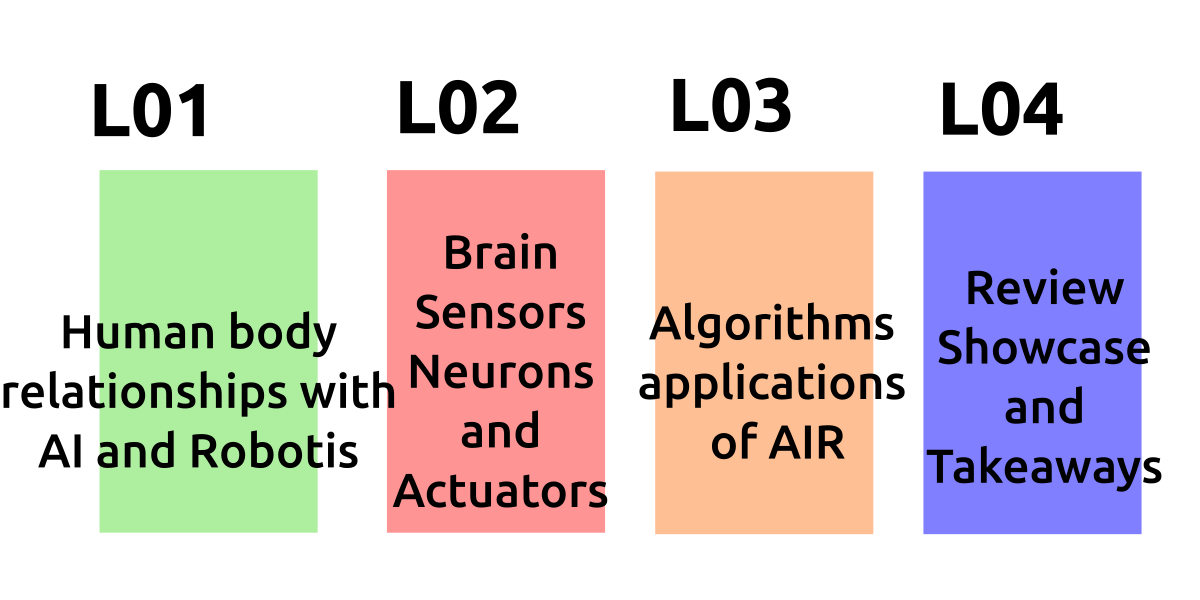
\includegraphics[width=\linewidth]{../figures/teaching-materials/versions/drawing-v00.png}
  \caption{(a) Spiral learning divided into lecture, virtual and physical laboratory and connected via project to next session \cite{tarik2017} (b) robot assembly and (c) block-like programming style.}
  %\Description{.}
  \label{fig:tm}
\end{figure}
 

% BLURS 
%Finding solutions together translate to social situations as well as it provides children with the foundations for decision making, logical reasoning, categorizing, analytical thinking, negotiation, and creativity. 
%In that way, AIR4Children's workshop integrates various hands-on activities where the children will develop different intellectual and social skills to incorporate into other areas of their lives.
%More specifically, such workshops are based on several Montessori principles such as: moving from the simple to the complex, the concrete to the abstract, the familiar to the unfamiliar and the general to the specific, as well as a mixed age group, where children can learn from each other.

%Using a variety of teaching materials that combine theory and practice, our workshop has the goal to create experiences to build children’s confidence, develop creativity, teamwork and curiosity.
%During these activities they are observed in order to: i) discover individual and team skills, ii) develop their talents, and iii) monitor their growth.  

%[Section to describe open teaching materials, perhaps using non-traditional education systems.]
%Serholt 2017 performed studies to quantify the social intereaction 
%between robots and children (i.e., gaze, verbal interaction, gestures, 
%and facial expressions). However robotics tutors are not yet to the point 
%to deal with complex child-robot interactions. 
%\cite{Serholt:2017}

\section{Conclusions and future work}
In this work, we coin the term AIR4Children as a project that aims to tackle aspects of inclusion, accessibility, transparency, equity, fairness and participation of children in the fields of AI and Robotics as well as to create teaching materials with a more child-centre approach for AI and Robotics.
We also touched on the open source projects in AI and Robotics as a corner stone for AIR4Children with the aim of minimise cost of the materials and made customised educational materials.  
We added our previous experience of few pilots since 2013 as way to narrow down the aims of AIR4Children.
Similarly, it has been presented the initial phases of AIR4Children that include piloting, implementing and refining workshops for children in the age range between 6 to 14 (to be implemented in Xicohtzinco, a town from Tlaxcala, M\'exico).
We also touched on the creation of curriculums following the philosophy of Montessori education, a non-traditional educational approach to help young audiences to develop skills to think creatively, with curiosity and open-minded and to develop a sense of wonder and joy for learning.

As a future work, AIR4Children aims to run workshops by the end of 2021 to put in practice educational material of child-centre AI and Robotics and to evaluate the impact on these fields to children, instructors, parents and their community. 

%% BLURS 
%Since children are going to learn and enter to this vast world of technology is in our responsibility to create open safe platforms and strategies where every children can enter and learn about AI, regardless of their personal situation, to avoid creating an “AI divide”. 
%To create a free safe space means the development and implementation of new AI policies focused on children, and the creation of digital public goods including open AI models, open software and so on.
%In our fast-evolving world towards technology is important to teach children what they are going to face when they grow up, unfortunately many children don’t have access to technology or the opportunity to learn about robotics and AI, and others, although they already know this type of technology, they don’t know how it works and how to create more of this technology which is really important towards the future. 
%This project aims for that goal, create a free space where we can help children know and comprehend the functionality of Robotics and AI so they can obtain the best of it and create even more technology, with a positive impact in society, regardless of their opportunities or status, we believe that every children has the potential to learn and create.

%% The acknowledgments section is defined using the "acks" environment
%% (and NOT an unnumbered section). This ensures the proper
%% identification of the section in the article metadata, and the
%% consistent spelling of the heading.
\begin{acks}
To Rocio Montenegro for her contributions and input as Montessori teacher. 
To Elva Corona for her contributions on giving vision to the goals of the project. 
To Marta P\'erez, Donato Badillo-Per\'ez and Antonio Badillo-Per\'e\ for their interest as initial testers of the project. 
To Leticia V\'azquez for her inputs as a teacher of teenagers. 
To Angel Mandujano for his help on the preparation of the software frameworks for the project. 
To Dago Cruz for his contributions on open source AI and Robotics.
To all of you of whom with the limited time were able to contribute to this work to make a bit more solid.
Thanks to Miguel Xochicale to orchestrate AIR4Children.
\end{acks}

%%
%% The next two lines define the bibliography style to be used, and
%% the bibliography file.
\bibliographystyle{ACM-Reference-Format}
\bibliography{../references/references}
%% \documentclass[conference]{IEEEtran}
\IEEEoverridecommandlockouts
% The preceding line is only needed to identify funding in the first footnote. If that is unneeded, please comment it out.
\usepackage{cite}
\usepackage{amsmath,amssymb,amsfonts}
\usepackage{algorithmic}
\usepackage{graphicx}
\usepackage{textcomp}
\usepackage{xcolor}
\def\BibTeX{{\rm B\kern-.05em{\sc i\kern-.025em b}\kern-.08em
    T\kern-.1667em\lower.7ex\hbox{E}\kern-.125emX}}

%=================================================================
%====ADDITIONAL PACKAGES & SETTINGS FROM THE ORIGINAL TEMPALTE====
\usepackage{import} % to use \import{../../../content-tex/}{abstract}
\usepackage{todonotes} % USAGE: \todo[inline]{is there a better example from X topic?}
\usepackage{lipsum}  % USAGE \lipsum[2-4]
\graphicspath{{../figures}} %goes to path: figures/
\newcommand{\etal}{\textit{et al. }} % \etal


\begin{document}

\title{
% Diversity, Equity, and Inclusion of Artificial Intelligence and Robotics for children %Fri  7 Jan 23:59:42 GMT 2022
%Piloting Inclusive Workshops of Artificial Intelligence and Robotics for children %Sat  8 Jan 00:12:35 GMT 2022
%Piloting Inclusive Artificial Intelligence and Robotics for Children %Sat 15 Jan 08:44:06 GMT 2022
%Piloting Diversity and Inclusion in Artificial Intelligence and Robotics for Children %Sat 15 Jan 10:33:54 GMT 2022
Piloting Diversity and Inclusion Workshops in Artificial Intelligence and Robotics for Children %Sun 16 Jan 13:14:45 GMT 2022
}

\author{

\IEEEauthorblockN{
    %1\textsuperscript{st} 
    air4children
    }
\IEEEauthorblockA{
    %\textit{dept. name of organization (of Aff.)} \\
    \textit{air4children: Artificial Intelligence and Robotics for Children}\\
    Xicohtzinco, M\'exico \\
    air4children@gmail.com
}

}

% \author{\IEEEauthorblockN{1\textsuperscript{st} Diego Coyotzi-Molina}
% \IEEEauthorblockA{\textit{dept. name of organization (of Aff.)} \\
% \textit{name of organization (of Aff.)}\\
% City, Country \\
% email address or ORCID}
% \and
% \IEEEauthorblockN{2\textsuperscript{nd} Rocio Montenegro}
% \IEEEauthorblockA{\textit{dept. name of organization (of Aff.)} \\
% \textit{name of organization (of Aff.)}\\
% City, Country \\
% email address or ORCID}
% \and
% \IEEEauthorblockN{3\textsuperscript{rd} Donato Perez-Badillo}
% \IEEEauthorblockA{\textit{dept. name of organization (of Aff.)} \\
% \textit{name of organization (of Aff.)}\\
% City, Country \\
% email address or ORCID}
% \and
% \IEEEauthorblockN{4\textsuperscript{th} Dago Cruz}
% \IEEEauthorblockA{\textit{dept. name of organization (of Aff.)} \\
% \textit{name of organization (of Aff.)}\\
% City, Country \\
% email address or ORCID}
% \and
% \IEEEauthorblockN{5\textsuperscript{th} Antonio Perez-Badillo}
% \IEEEauthorblockA{\textit{dept. name of organization (of Aff.)} \\
% \textit{name of organization (of Aff.)}\\
% City, Country \\
% email address or ORCID}
% \and
% \IEEEauthorblockN{6\textsuperscript{th} Leticia Vazquez}
% \IEEEauthorblockA{\textit{dept. name of organization (of Aff.)} \\
% \textit{name of organization (of Aff.)}\\
% City, Country \\
% email address or ORCID}
% }

\maketitle

\begin{abstract}
This document is a model and instructions for \LaTeX.
We presents our findings on the first pilot workshop (a) to promote diversity and inclusion; and (b) to encourage children to discover and increase their interest in AI and Robotics.
This and the IEEEtran.cls file define the components of your paper [title, text, heads, etc.]. 
*CRITICAL: Do Not Use Symbols, Special Characters, Footnotes, or Math in Paper Title or Abstract.
\lipsum[2]
\end{abstract}

\begin{IEEEkeywords}
    Open Educational Resources, Educational robots
\end{IEEEkeywords}

%%%%%%%%%%%%%%%%%%%%%%%%%%%%%%%%%%%%%%%%%
%%%%%%%%%%%%%%%%%%%%%%%%%%%%%%%%%%%%%%%%%
\section{Introduction}
%Guarantee security, accessibly and human dignity are considered the pillars for inclusivity.
Accessible and affordable technology in conjuntion with open educational resources can promote equal opportunities for childhood education \cite{yoshie2021-unesco}.
However, teaching state-of-the-art technologies such as Artificial Intelligence and Robotics, AIR, is a current challenge for low-income and often politically or culturally marginalized countries.
Additionally, creating the right environment to promote inclusivity and diversity to teach AIR has been little investigated. 
Astobiza \etal 2019. for instance, reported the need of collaborations between industry and a multidisciplinary group of researchers to address concerns on the paradigm of inclusivity in robotics \cite{MonasterioAstobiza2019}.
In that sense, Astobiza \etal suggested that inclusive robotics should be based on two points: "1) they should be easy to use, and 2) they must contribute to making accessibility easier in distinct environments" \cite{MonasterioAstobiza2019}.
Peixoto \etal in 2018 reported the use of robots as tool to promote diversity leading to improve competences in communication, teamwork, leadership, problem solving, resilience and entrepreneurship \cite{PeixotoCastro2018, PeixotoGonzalez2018}. 
Recently, Pannier \etal in 2020 pointed out the challenges of increasing the  participation of women and underrepresented minorities in the areas of Mechatronics and Robotics Engineering as well as the creation of community of educators to promote diversity and inclusion \cite{Pannier2020}.
Similarly, Pannier \etal mentioned that the prevalence of free and open-source software and hardware made mechatronics more accessible to a diverse group of population.
Pannier \etal also touched on the importance of offering workshops to different range of underrepresented students leading to inspire other programs and to create outreach activities for students, trainers and workshops \cite{Pannier2020}.
Recently, Montenegro \etal in 2021 introduced air4children, Artificial Intelligence and Robotics for Children, as a way (a) to address aspects for inclusion accessibility, equity and fairness and (b) to create affordable child-centred materials in AI and Robotics (AIR) in low-income countries \cite{montenegro2021air4children}. 
In that sense, another challenge is organising workshops where little is known about the demographics, education and socio-economical varibles that impact such communities.
For instance, Xicohtzinco, Tlaxcala M\'exico, is a town of a total population of 14,197 (6762 males and 7435 females) based on the INEGI's census 2020.
However, the census do not provide number of schools but based on the current habitants, we understand that that there are three public schools including kinder-garden, primary, secondary and high-school; and three private schools including primary and secondary schools. 
% NOT QUITE SURE ABOUT THIS SPECULATIONS:
%What it is not known from the 2020 census is the education levels of the population but our anecdotal experience and from current habitants can tell that the population is a mixture of young professionals and working class population.
That said, we hypothesed that piloting workshops of air4chidren in a town such as Xicohtzinco might led us to have better understanding of the needs and challenges of promoting diversity and inclusion of state-of-the-art technologies with open education resources.

This short paper is organised as follows:
Section II presents Tools to promote Diversity and Inclusion in AI and Robotics for chldren.
Section III presents the design of workshops for children from 6 to 8 years old.
Section IV presents outcomes of a four lessons pilot workshop for 14 children and the help of three instructors and three supervisors. 
We present results of the workshops and finalise it with conclusions and future work.

%BLURS
% in Artificial Intelligence and Robotics (AIR).
% to encourage children to discover and increase their interest in 
% to promote of air4children and to create the inclusive and diversity environments might led us to have better understanding of the current needs and might provide with further evidence 
% of the real needs of the community. 
%we design and pilot workshops of air4children to test how children of different ages and genders and instructors engage to create an environment of diversity and inclusion. 


%%%%%%%%%%%%%%%%%%%%%%%%%%%%%%%%%%%%%%%%%
%%%%%%%%%%%%%%%%%%%%%%%%%%%%%%%%%%%%%%%%%
\section{Tools to promote Diversity and Inclusion in AI and Robotics for chldren}
\todo[inline]{MX: this section/subsection requires to be refined by adding perpahs other references and align it to air4children}

\subsection{Free and open-source software, open-source hardware and open educational resources}
Recently, Montenegro \etal presented examples to create educational resources aimed to be "affordable, educational and fun", such examples are Otto DIY -- an educational open source robot and JetBot platform -- open source educational robot to create new AI projects \cite{montenegro2021air4children}.
In that sense, Otto Humanoid is a good option for our work because of its affordability costing of 200 EUROS, a block diagram programming interface, the multiple sensors and actuators (servos and LCD matrix display) aligned with open-source software and hardware principles \cite{OttoDIY:2016}.
Similarly, Open Educational Resources (OER) aiming to provide "teaching and learning materials that are available without access fees" seems to be a right direction to afford innovation through OER-enabled pedagogy \cite{Clinton-Lisell2021}.
Wiley \etal in 2014 stated that one of the benefits of OERs is to make course development process quicker and easier but also highlighting the challenges of making OER material for people easier to find but with the challenge of making financially self-sustainable programs among many other difficulties \cite{Wiley2014}.

\subsection{Alternative education programs with new technologies}
Alternative education programs such as Montessori, Waldorf and Regio Emilia considers children as active authors of their own development \cite{edwards2002}.
These programs have been well adopted internationally; however Edwards \etal pointed out the schools deriving from the same philosophy might also need to observe teacher-child interactions, its environments and interview to the past and present parents and children \cite{edwards2002}.
Similarly, in the last 5 years such programs are starting to include topics on AI, robotics and computational thinking into their curriculum \cite{elkin2014, Aljabreen2020}.
For instance, Aljabreen pointed out the adoptions of new technologies and how early child education is re-conceptualised \cite{Aljabreen2020}. 
Elkin et al. in 2014 explored the how robots can be used in the Montessori curriculum \cite{elkin2014}.
Similarly Elkin et al. posed the question on the revision of new curriculums that include technology should not deviate from the main purpose of the Montessori classroom \cite{elkin2014}.
Drigas and Gkeka in 2016 reviewed the application of information and communication technologies in the Montessori Method, mentioning the Manipulatives, as objects to develop motor skills or understand mathematical abstractions, are based on cultural areas, language, mathematics and sensoria but little to none on technological areas \cite{DrigasGkeka2016}.
Drigas and Gkeka reviewed Montessori materials of the 21st century where interactive systems with sounds and lights, touch application to enhance visual literacy or the development of computational thinking and constructions of the physical world \cite{DrigasGkeka2016}.
These indicate that the incorporation of such manipulatives with the use of robotics might led to reach scenarios to explore motor skill development, visualisation and computational thinking. 
Recently, Scippo and Ardolino reported a longitudinal study of the use of computational thinking in five years participants of primary school in a Montessori school \cite{ScippoArdolino2021}
Scippo and Ardolino pointed out the importance of alignment of the Montessori material with the computational thinking activities. 

That said, previous authors stated various challenges on the incoporation of new technologies into their curriculum posing more questions on creating curriculims that should be more accessible to a diverse group of population as it is done in the case of open educational resources.


%%%%%%%%%%%%%%%%%%%%%%%%%%%%%%%%%%%%%%%%%
%%%%%%%%%%%%%%%%%%%%%%%%%%%%%%%%%%%%%%%%%
\section{Designing Diversity and Inclusion Workshops}
To design diversity and inclusive workshops we were considered the six ideas discussed in "Ensuring education and Inclusive Learning for Educational Recovery 2021" \cite{opertti2021-unesco} and 
‘Concrete to abstract’ concept within the Montessori philosophy \cite{MontessoriBOOK1969}.
In one hand, we considered the six ideas to ensuring and inclusive learning summarised as:
(1) personalisation of education including the recognition of specific learning expectations and needs,
(2) designing inclusive, emphatic and participatory curriculum for an plural and open participation of a diversity of actors and institutions,  
(3) appropriation of technology as a community resource to strength ties between students, educators, families and communities,  
(4) empowering knowledge, learning, collaboration, trust and listening among peers, and
(5) the visualisation of schools as lifelong learning spaces.
On other hand, the workshop were planned to develop concepts and skills using 'concrete' concept with hands-on learning materials to make abstract concepts clearer as it is taught in Montessori education \cite{MontessoriBOOK1969}. 

That said, with the combination of Open Educational Resources, alternative education programs and the six ideas, we designed a four lesson workshop with two-fold aims:
(a) to promote diversity of and inclusion to children to teach AI and Robotics and 
(b) to encourage children to discover and increase their interest in AI and Robotics. Figure \ref{fig:curriculum} presents four lessons of the workshops.

\begin{figure}[t]
    % \centerline{\includegraphics[width=\linewidth]{figures/curriculum.png}}  %%OVERLEAF
    \centerline{\includegraphics[width=\linewidth]{curriculum-design/versions/drawing-v01.png}}  %%GITHUB
    \caption{Curriculum for four lessons (L01 to L04). 
    Lesson 01 introduce the course, 
    lesson 02 provides the basics of anatomy, 
    lesson 03 covers algorithms, and 
    lesson 04 wrap-up and showcase the project of children.
    }
    \label{fig:curriculum}
\end{figure}

\paragraph{Lesson 01: Breaking the ice and motivations} 
The educational goal for this lesson was to develop the children’s curiosity about AI and Robotics while emphasizing the importance of interpersonal connections that will evolve into a collaboration work for the following lessons.
That said, this lesson started with a recreational activity where each student and teacher introduced themselves with name, favorite food and a superpower or ability that we would like to have and that was related to robots. This lesson also covers basic concepts and examples of AI and Robotics in different fields and daily life, how the brain works and how the human senses and body parts relates to the way a robot is built and how it works and perform activities.

\paragraph{Lesson 02: Human senses and coding my first robot} 
The main purpose of this lesson was to understand fundamentals of Robotics. 
Children began to work with more abstract concepts, developing problem-solving skills as well as cooperatively working relationships. 
The first activity, outside of the classroom, was a true or false game, were the teacher told a sentence about AI and Robotics, and the children jumped in front of a rope if the sentence was true, or if the sentence was false, the kids jumped behind of the rope.
In the second activity, the instructor explain about the human senses and their relationship with inputs and outputs. After that, instructors explain examples of sequences and codes. 
In the last activity, participants were asked to sort out tangram in a group in which a leader of the group provide instructions to the team-mates as an analogy of coding a robot with algorithms.

\paragraph{Lesson 03: Playing with reaction-action activities} 
The educational goal of this lesson is to cover the concept of the effect of causes and consequences with daily life examples and the computational thinking of robots.
Hence, this lesson start with a match game consisting of figures and shadow’s figures where participants develop their comparing skills to match similar or different robots.
This lesson covered points on how robot works with sensors, processors, actuators and programming. 
The “find the effect” activity was also introduced where participants have to relate pictures of cause and consequences, for example “the cause is the rain and the consequently is a rainbow”.
Afterwards, we worked with the Otto humanoids in which we programmed the sensor presence for that robot moves, dances and that emit texts with the 8x8 matrix.

\paragraph{Lesson 04: Develop your own AIR}
The four lesson aimed to summaries what was covered in the previous lessons emphasising the relationship of the human body anatomy (brain, neurons and body parts) with humanoid robots (computer, sensors and actuators).
This lesson covered real-word application of AI and Robotics including medicine, spacial robotics and smart cities. 
Three projects were prepared to be introduced to each team in which every participant have a role. 
Each team prepare a short speech of their application using AI and Robotics. 
%%%%%%%%%%%%%%%%%%%%%%%%%%%%%%%%%%%%%%%%%
%%%%%%%%%%%%%%%%%%%%%%%%%%%%%%%%%%%%%%%%%
\section{Piloting Diversity and Inclusion Workshops}
To pilot the workshop, we invited 14 (6 female and 8 male) participants with range of age from 6 to 11 years old (average age of 7.64).
Similarly, three instructors with 3 years of experience in teaching and two coordinators with 10 years of teaching experience volunteered to deliver four lessons.
Originally, each lessons was planned to be 90 minutes but we did not consider breaks or perhaps the children's energy levels of some of the participants to which in the second to four lesson a 15 minutes break was incorporated.
We surveyed children with questions about their understanding and feelings towards different type of robots to find out that some of the children were not in the age to read, to which we support them. 
Although the survey contained only 10 questions, we decided to made use of 10 minutes at the start of each lesson to complement all the questions.

Figure \ref{fig:pilot} illustrates instructors and children during interactive activities. 
\begin{figure}[tbp]
    % \centerline{\includegraphics[width=\linewidth]{figures/workshop.png}} %%OVERLEAF
    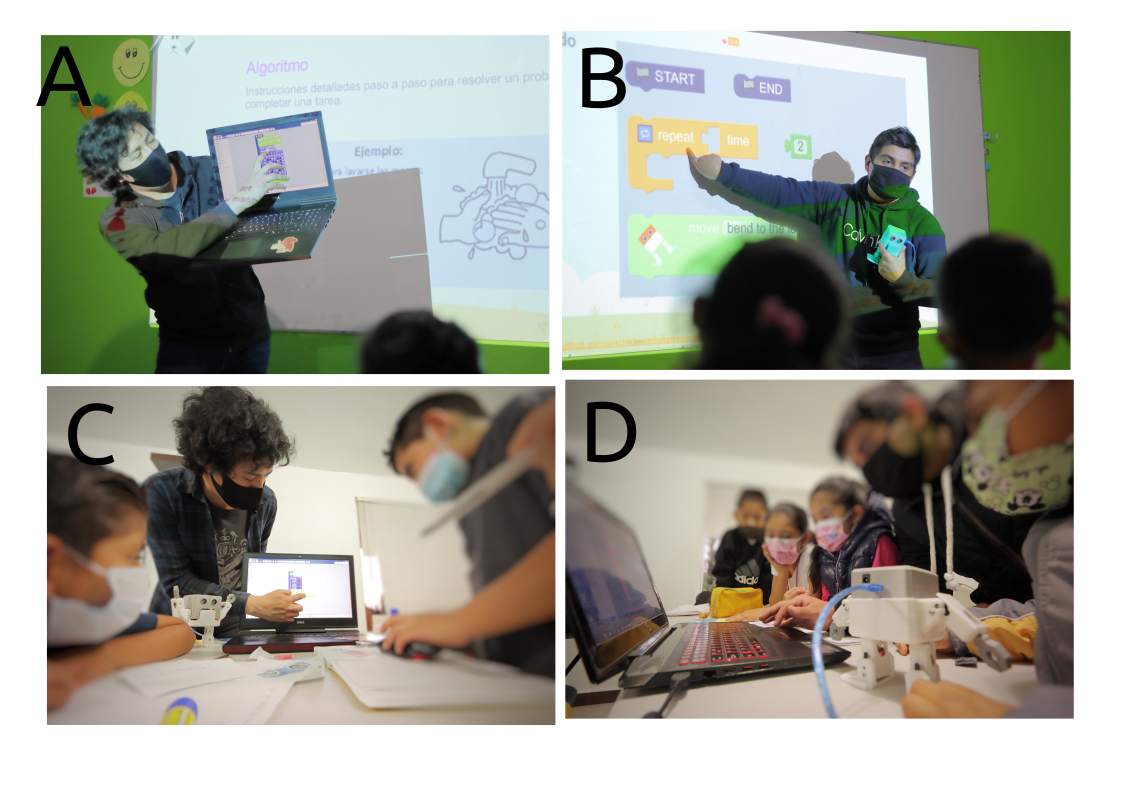
\includegraphics[width=\linewidth]{piloting-workshops/versions/drawing-v00.png} %%GITHUB
    \caption{
        Instructors demonstrating basics of AI and Robotics (A, and B). 
        Children engaging with robots, classmates and instructors (B, and C).
        }
    \label{fig:pilot}
\end{figure}

As the lessons progress the children incorporate the knowledge they gained and are able to put concepts together. 
A show case of their final work promoted a sense of achievement in the children working not only with their mind but also with their social emotional well-being. 


% \begin{table}[htbp]
%     \caption{Table Type Styles}
%     \begin{center}
%     \begin{tabular}{|c|c|c|c|}
%     \hline
%     \textbf{Table}&\multicolumn{3}{|c|}{\textbf{Table Column Head}} \\
%     \cline{2-4} 
%     \textbf{Head} & \textbf{\textit{Table column subhead}}& \textbf{\textit{Subhead}}& \textbf{\textit{Subhead}} \\
%     \hline
%     copy& More table copy$^{\mathrm{a}}$& &  \\
%     \hline
%     \multicolumn{4}{l}{$^{\mathrm{a}}$Sample of a Table footnote.}
%     \end{tabular}
%     \label{tab1}
%     \end{center}
% \end{table}
    


%%%%%%%%%%%%%%%%%%%%%%%%%%%%%%%%%%%%%%%%%
%%%%%%%%%%%%%%%%%%%%%%%%%%%%%%%%%%%%%%%%%
\section{Conclusions and future work}
In this paper, we investigate the challenges of Diversity and Inclusion to teach "Artificial Intelligence and Robotics for Children" with open educational resources and principles of Montessori education. 
For the design and the pilot of the workshop, we invited 14 children of an average age of 7.64 years old participated of the community of Xicohtzinco Tlaxcala Mexico.
The workshops were free of cost as a way encourage participation of anyone. 
During the pilot workshop, children were enthusiastic about learning the fundamentals for AIR by building, coding, designing and playing with open-sourced robots. The instructors embraced the different set of skills each child had by working in small groups and supporting the students during the process. These lessons intended to remain beyond the learning of a single concept and contribute to develop a skill the children can take and apply to other areas in their life.
However, we noted that grouping children of four participants with one instructor was not creating an engaging experience as each group has only one robot and one computer and the space and number of participants was leaving sometimes one participant outside of the reachable robot-computer setup.
As a future work, we are planing to organise another workshop in the four quart of the 2022 where we will consider 10 lessons distributed in four weeks with we will invite more participants.
For curriculum of the workshops, we will improve the interactivity of the participants and create more engaging and inclusive activities. We will incorporate a similar approach of the synthesis program which aim is to cultivate student voice, strategic thinking and collaborative problem solving \cite{synthesis2022}.
%started in 2014 with Josh Dahn and support of Elon Musk, 



\section*{Acknowledgment}
To Rocio Montenegro for her contributions with the design of the Montessori curriculum for the workshops.
To Marta P\'erez, for their support in organising the pilot of the workshops.
To Diego Donato Badillo-Per\'ez and Antonio Badillo-Per\'e\ for volunteering as instructors of the workshops.
To Leticia V\'azquez for her support with the logistics and feedback to improve the workshops.
To Adriana Fortiz-Perez for her contributions and discussion to prepare draft surveys for the parents and children. 
To Elias Mendes for his support and feedback on the hardware design of the robot.
To Dago Cruz for his feedback and discussions on the design of the workshops.
To Angel Mandujano, Elva Corona and others who have contributed with feedback and support to keep iterating the project of AIR4children. 


\section*{Contributions}
Antonio Perez-Badillo: Contributing to design and write up of lesson 02.
Dago Cruz:
Diego Coyotzi-Molina: Contributing to design and write up of lesson 03.
Donato Perez-Badillo: Contributing to design and write up of lesson 01.
Leticia Vazquez: Write up and refinement of the conclusions.
Miguel Xochicale: Contributing to create the template, drafting, write-up, edition, and submission of the paper. 
Rocio Montenegro: Contributing to the write up of designing and piloting workshops. 

\bibliographystyle{IEEEtran}
% \bibliography{references} %%OVERLEAF
\bibliography{../references/references} %%GITHUB


\end{document}
 %% uncomment for arxiv version

\end{document}
\endinput
%%
%% End of file `sample-sigconf.tex'.
